\section{Circuit design} \label{section: circuit design}
\subsection{Softwares used}
We used the following softwares to design and simulate the circuit:
\subsubsection{Matlab}
We used Matlab to simulate the input signal of the sensor. Matlab is a programming and numeric computing platform used by millions of engineers and scientists to analyze data, develop algorithms, and create models. Matlab allows matrix manipulations, plotting of functions and data, implementation of algorithms, creation of user interfaces, and interfacing with programs written in other languages.
\subsubsection{LtSpice}
We used LtSpice to simulate the circuit and test it. LtSpice is a high performance SPICE simulator, schematic capture and waveform viewer with enhancements and models for easing the simulation of analog circuits.

\subsection{The input signal}
The signal we are trying to measure is the force applied to the foot. We assume that the frequency of the force applied to the foot is about 1 Hz and the maximum force applied to the sensor is about 1000 N. We also assume that the sensor has a white noise with a standard deviation of 0.01 V and the urban electric noise frequency is about 50 Hz with a standard deviation of 0.1 V. We also assume that the input signal has a shape of sine wave. Thus we have:
\begin{align}
     & V_{Front} = 0.0032  sin(2\pi t) + 0.1 sin(100 \pi t) + n(t)        \\
     & V_{Back} = 0.0032  sin(2\pi t + \pi/2) + 0.1 sin(100 \pi t) + n(t)
\end{align}
Where $V_{Front}$ is the voltage generated by the piezoelectric attached to the front of the foot and $V_{Back}$ is the voltage generated by the piezoelectric attached to the back of the foot and $n(t)$ is the white noise with a standard deviation of 0.001 V.
The signal simulated in Matlab is shown below:
\begin{figure}[H]
    \centering
    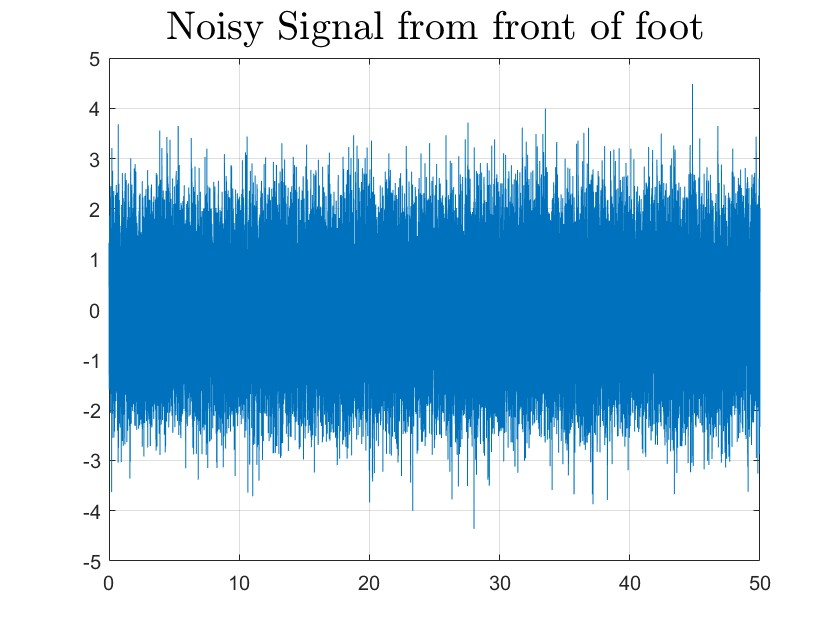
\includegraphics[width=0.8\textwidth]{../Report/Figures/2.CircuitDesign/InputSignal_WithNoise.jpg}
    \caption{Realistic input signal simulated in Matlab.}
\end{figure}

\subsection{The circuit}
The block diagram of the circuit is shown below:
\begin{figure}[H]
    \centering
    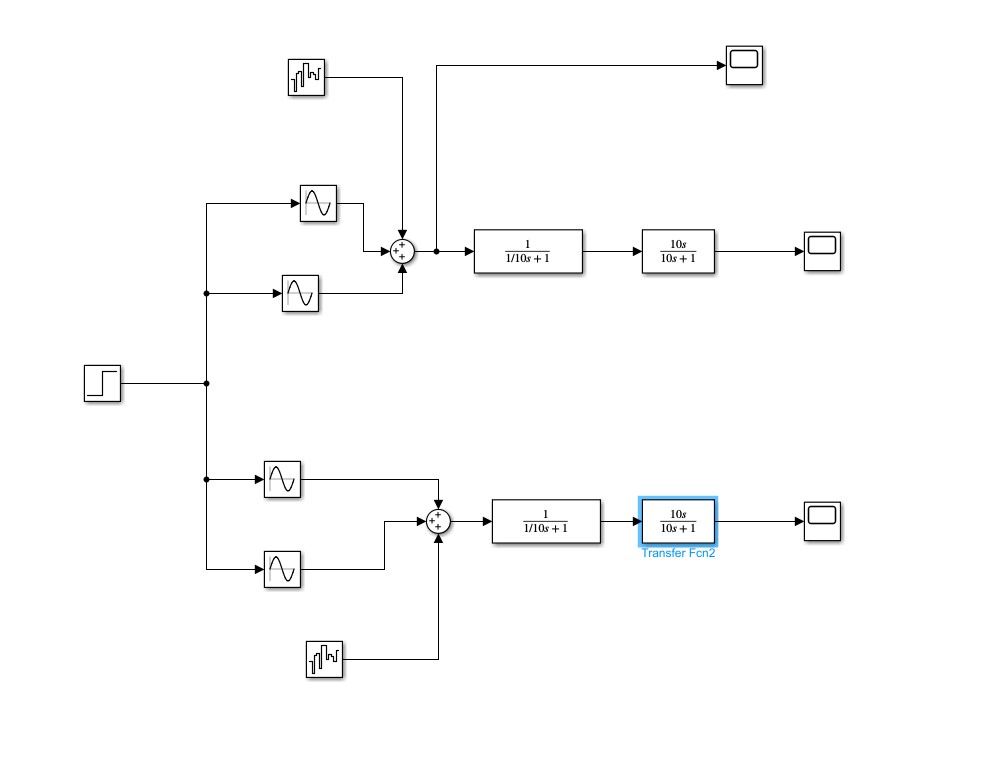
\includegraphics[width=0.8\textwidth]{../Report/Figures/2.CircuitDesign/BlockDiagram.jpg}
    \caption{The block diagram of the circuit.}
\end{figure}
Block diagram of the circuit contains 2 important parts:
\begin{itemize}
    \item \textbf{The High pass filter:} A high-pass filter (HPF) is an electronic filter that passes signals with a frequency higher than a certain cutoff frequency and attenuates signals with frequencies lower than the cutoff frequency. The amount of attenuation for each frequency depends on the filter design. A high-pass filter is usually modeled as a linear time-invariant system. It is sometimes called a low-cut filter or bass-cut filter in the audio domain. High-pass filters have many uses, such as blocking DC from circuitry sensitive to non-zero average voltages or radio frequency devices. They can also be used in conjunction with a low-pass filter to produce a bandpass filter.
    \item \textbf{The low pass filter:} A low-pass filter is a filter that passes signals with a frequency lower than a selected cutoff frequency and attenuates signals with frequencies higher than the cutoff frequency. The exact frequency response of the filter depends on the filter design. The filter is sometimes called a high-cut filter, or treble cut filter in audio applications. A low-pass filter is the complement of a high-pass filter.
\end{itemize}
Trnasfer function for a high pass filter is given by:
\begin{equation}
    H(s) = \frac{s}{s + \omega_{c}}
\end{equation}
Where $\omega_{c}$ is the cutoff frequency.\\
Trnasfer function for a low pass filter is given by:
\begin{equation}
    H(s) = \frac{\omega_{c}}{s + \omega_{c}}
\end{equation}
Where $\omega_{c}$ is the cutoff frequency.\\
Fpr the perfrence of the cutoff frequency, we chose $\omega_{c} = 2 \pi Hz$.\\
Thus desired transfer function for the high pass filter is given by:
\begin{equation}
    H(s) = \frac{s}{s + 2 \pi} \rightarrow R = 1 k\Omega, C = 0.300 \mu F
\end{equation}
And desired transfer function for the low pass filter is given by:
\begin{equation}
    H(s) = \frac{2 \pi}{s + 2 \pi} \rightarrow R = 1 k\Omega, C = 0.300 \mu F
\end{equation}
\subsubsection{The high pass filter}
The high pass filter is shown below:
\begin{figure}[H]
    \centering
    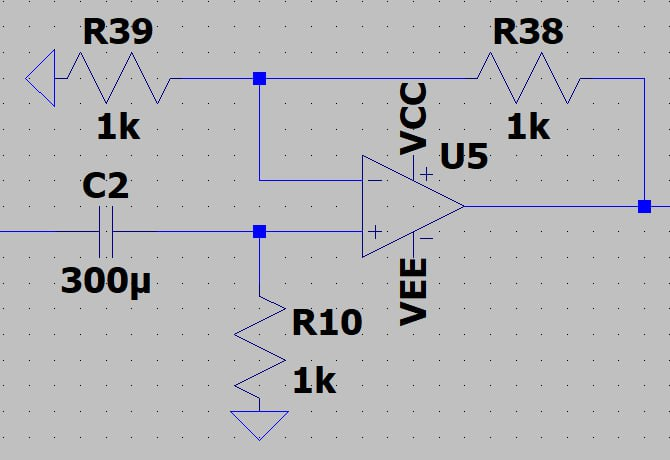
\includegraphics[width=0.6\textwidth]{../Report/Figures/2.CircuitDesign/HighPassFilter.jpg}
    \caption{The high pass filter.}
\end{figure}
The high pass filter is designed to filter the urban electric noise. The transfer function of the high pass filter is given by:
\begin{equation}
    H(s) = \frac{s}{s + 2 \pi}
\end{equation}

\subsubsection{The low pass filter}
The low pass filter is shown below:
\begin{figure}[H]
    \centering
    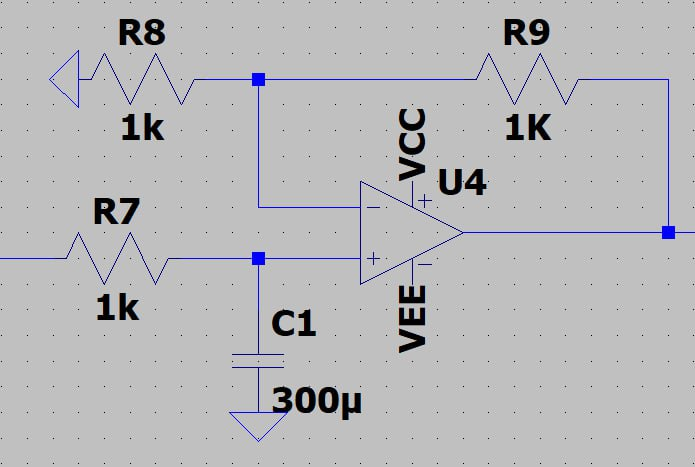
\includegraphics[width=0.6\textwidth]{../Report/Figures/2.CircuitDesign/LowPassFilter.jpg}
    \caption{The low pass filter.}
\end{figure}
The low pass filter is designed to filter the white noise. The transfer function of the low pass filter is given by:
\begin{equation}
    H(s) = \frac{2 \pi}{s + 2 \pi}
\end{equation}

\subsubsection{The Instrumentation amplifier}
The instrumentation amplifier is shown below:
\begin{figure}[H]
    \centering
    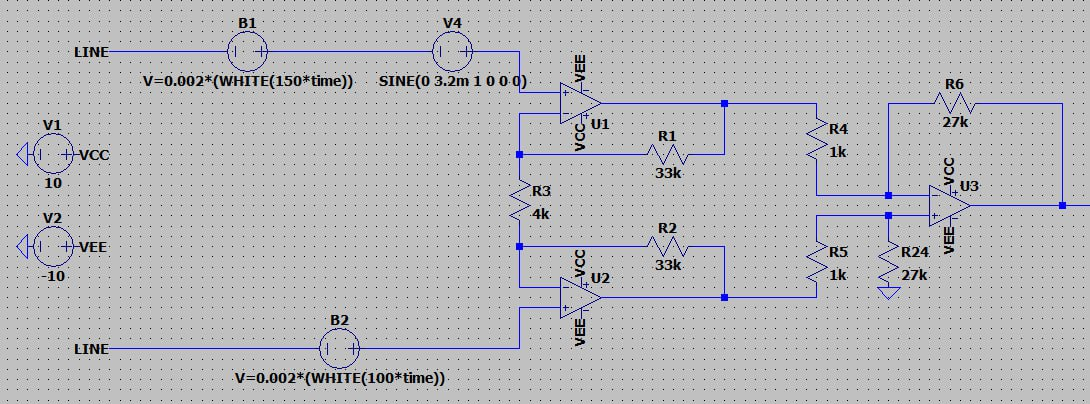
\includegraphics[width=0.9\textwidth]{../Report/Figures/2.CircuitDesign/InstrumentationAmplifier.jpg}
    \caption{The instrumentation amplifier.}
\end{figure}
The instrumentation amplifier is designed to amplify the difference between the two voltages. The gain of the amplifier is given by:
\begin{equation}
    A_{d} = \frac{V_{o}}{V_{1} - V_{2}} = (1 + 2 \frac{R_{1}}{R_{3}}) \frac{R_{6}}{R_{4}} = (1+\frac{33}{4})\times \frac{27}{1} = 9.25 \times 27 = 250
\end{equation}


\subsubsection{The summing amplifier}
The summing amplifier is shown below:
\begin{figure}[H]
    \centering
    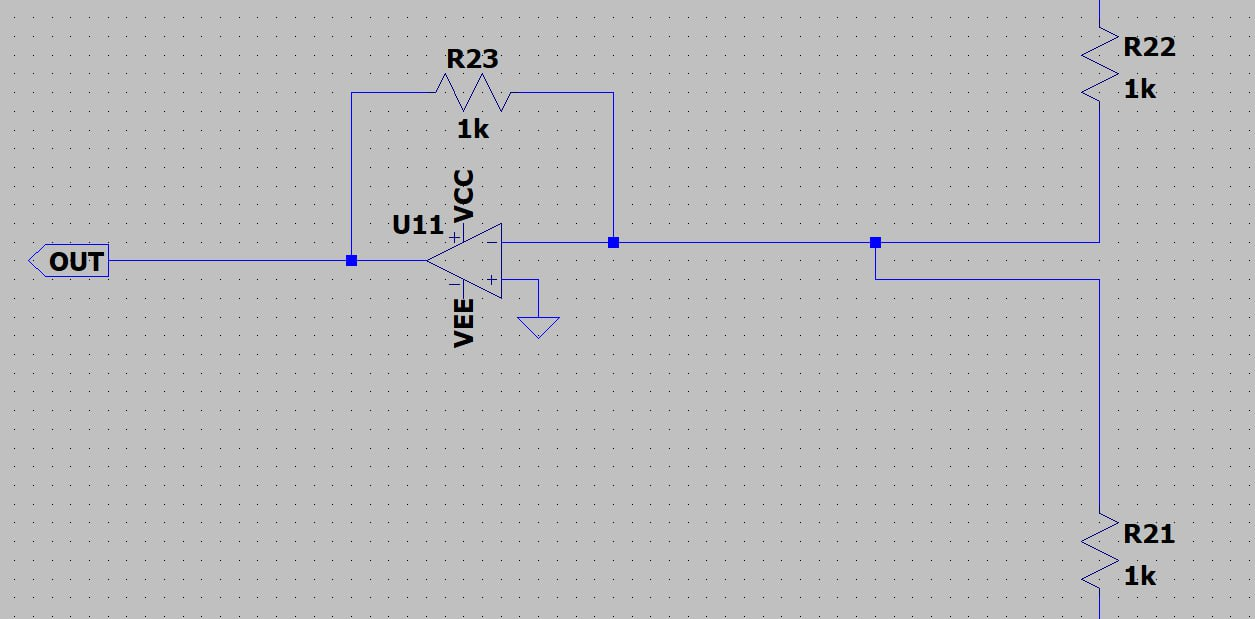
\includegraphics[width=0.7\textwidth]{../Report/Figures/2.CircuitDesign/SummingAmplifier.jpg}
    \caption{The summing amplifier.}
\end{figure}
The summing amplifier is designed to sum the output of the instrumentation amplifiers after passing through the low pass and high pass filters. The gain of the amplifier is given by:
\begin{equation}
    A_{d} = \frac{V_{o}}{V_{in}} = - \frac{R_{23}}{R_{21}} = - \frac{1 k\Omega}{1 k\Omega} = -1
\end{equation}


\subsubsection{The circuit designed to measure the force applied to the foot}
The circuit designed to measure the force applied to the foot is shown below:
\begin{figure}[H]
    \centering
    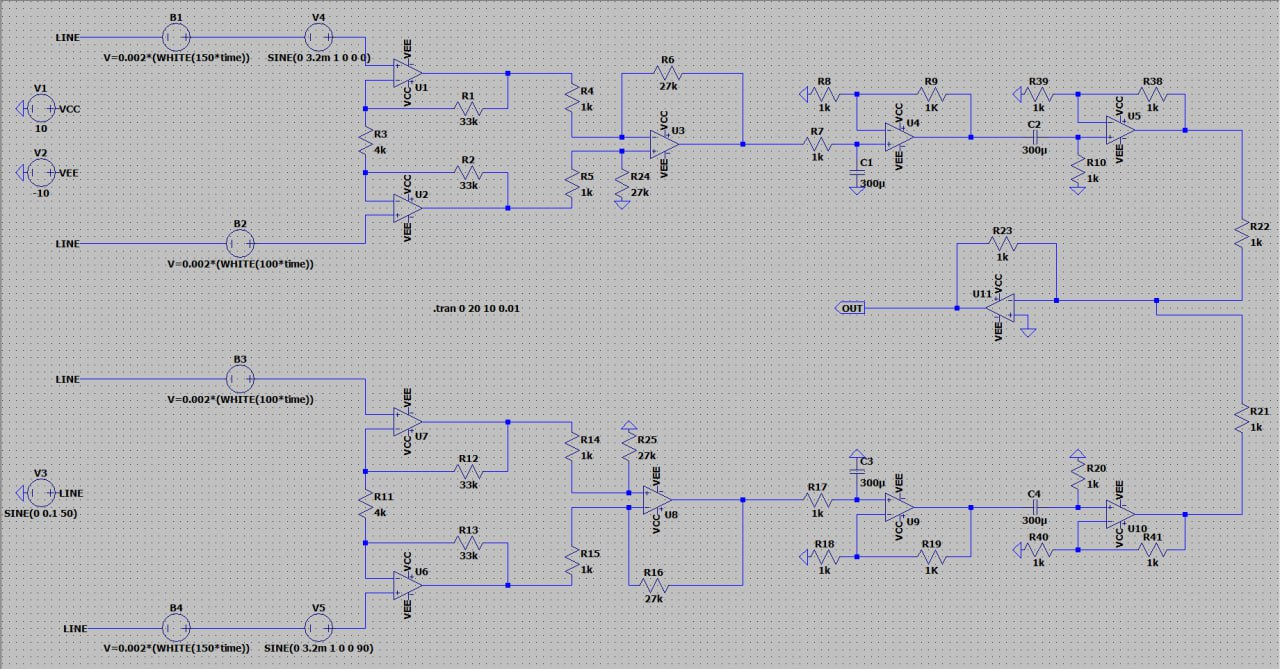
\includegraphics[width=0.7\textwidth]{../Report/Figures/2.CircuitDesign/Circuit.jpg}
    \caption{The circuit designed to measure the force applied to the foot.}
\end{figure}
The circuit is designed to measure the force applied to the foot. The output of the circuit is the voltage generated by the piezoelectric attached to the front of the foot and the piezoelectric attached to the back of the foot. The output of the circuit is given by:
\begin{equation}
    V_{o} = - (V_{Front} + V_{Back})
\end{equation}

\subsection{The simulation}
The simulation of the circuit is shown below:
\begin{figure}[H]
    \centering
    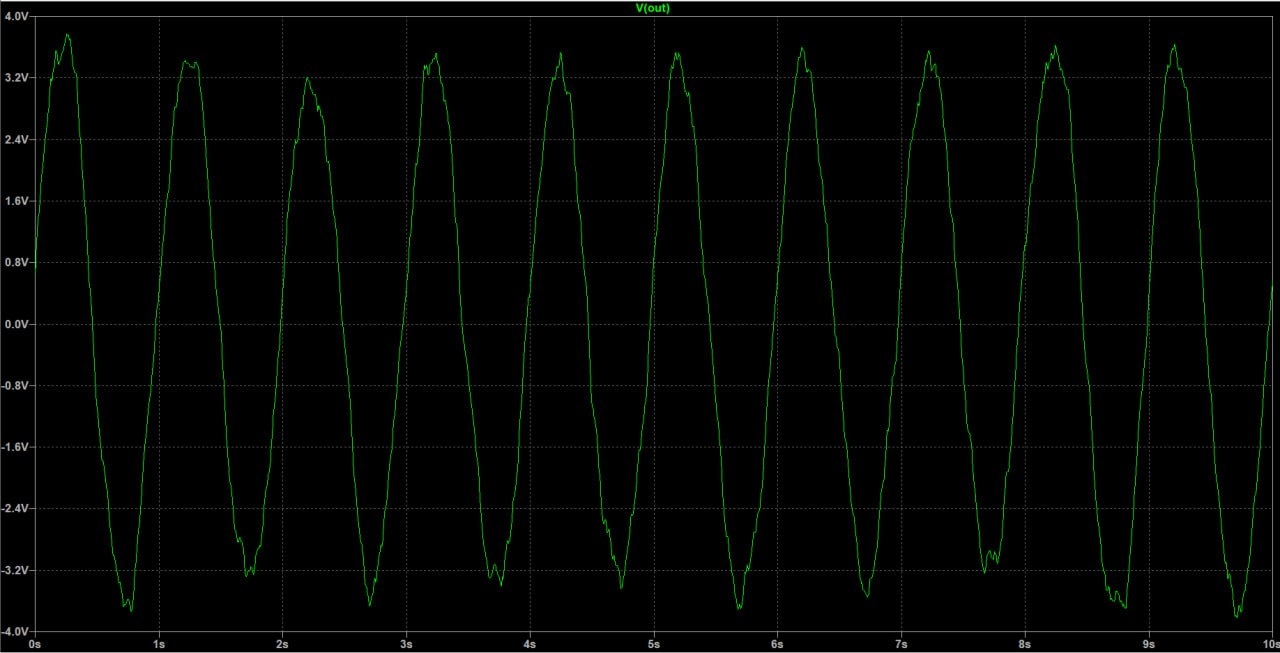
\includegraphics[width=0.9\textwidth]{../Report/Figures/3. Result/rsult.jpg}
    \caption{The simulation of the circuit.}
\end{figure}

Maximum output voltage is about 3.4 V and the minimum output voltage is about -3.4 V. The output voltage is the voltage generated by the piezoelectric attached to the front of the foot and the piezoelectric attached to the back of the foot for a man weighting 100 kg.\\
